% !TeX root = surprises.tex

\chapter{The Five-Color Theorem}\label{c.five}

%%%%%%%%%%%%%%%%%%%%%%%%%%%%%%%%%%%%%%%%%%%%%%%%%%%%%%%%%%%%%%%

Karten verwenden Farben, um eine Region von einer anderen zu unterscheiden, indem sie dafür sorgen, dass benachbarte Regionen mit unterschiedlichen Farben eingefärbt werden. Im Jahr 1852 stellte Francis Guthrie fest, dass eine Karte der Grafschaften Englands mit nur vier Farben eingefärbt werden konnte.
Die Behauptung, dass vier Länder ausreichen, um eine beliebige ebene Karte einzufärben, wird als \emph{Vier-Farben-Theorem} bezeichnet und wurde erst 1976 von Kenneth Appel und Wolfgang Haken bewiesen. Sie wendeten ausgeklügelte mathematische Argumente an, um zu zeigen, dass, wenn es ein Gegenbeispiel gibt (eine Karte, die mehr als vier Farben benötigt), diese mit einer von $1834$ Konfigurationen verbunden sein muss. Anschließend überprüften sie diese Konfigurationen mit einem Computer.

Während das Vier-Farben-Theorem extrem schwierig zu beweisen ist, sind die Beweise für das Fünf- und Sechs-Farben-Theorem relativ einfach (Abschnitte ~\ref{s.six-color}, ~\ref{s.five-color}). Auf dem Weg zum Beweis dieser Theoreme definieren wir planare Karten und Graphen (Sect.~\ref{s.planar}), beweisen die Eulersche Formel (Sect.~\ref{s.euler}) und zeigen, dass ein planarer Graph Scheitelpunkte haben muss, deren Grad kleiner oder gleich fünf ist. In Sect.~\ref{s.nonplanar} wird die Eulersche Formel verwendet, um zu zeigen, dass zwei Graphen nicht planar sind.

1879 veröffentlichte Alfred B. Kempe einen Beweis des Vier-Farben-Satzes, aber 1890 zeigte Percy J. Heawood, dass der Beweis falsch ist. In Sect.~\ref{s.kempe} präsentieren wir Kempes fehlerhaften Beweis und Heawoods Beweis, dass er nicht korrekt ist.

\section{Flächige Karten und Diagramme}\label{s.planar}

\begin{definition}
Eine \textit{planar map} ist eine Menge von Regionen in der Ebene, die durch Grenzen getrennt sind. Eine \textit{coloring} einer Karte ist eine Zuweisung einer Farbe zu jeder Region, so dass Regionen, die eine Grenze teilen, unterschiedliche Farben zugewiesen werden.
\end{definition}

Abbildung~\ref{f.five-planar-map-five} zeigt eine fünffarbige Darstellung einer ebenen Karte mit zehn Regionen.
Abbildung~\ref{f.five-planar-map-four} zeigt eine vierfarbige Darstellung der gleichen Karte.

\begin{figure}[t]
\begin{minipage}{.45\textwidth}
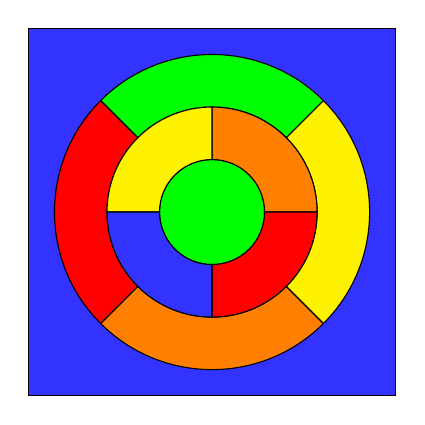
\begin{tikzpicture}[scale=.667]
\draw[fill=blue!80] (-3.5,-3.5) rectangle +(7,7);

\draw[fill=green] (0:1) 
  arc [start angle=0,  end angle=360, radius=1];

\draw[fill=green] (45:2) --
      (45:3)  arc[start angle=45,  end angle=135, radius=3] --
      (135:2) arc[start angle=135, end angle=45,  radius=2];
\draw[fill=orange] (-45:2) --
      (-45:3)  arc[start angle=-45,  end angle=-135, radius=3] --
      (-135:2) arc[start angle=-135, end angle=-45,  radius=2];
\draw[fill=yellow] (45:2) --
      (45:3)  arc[start angle=45,  end angle=-45, radius=3] --
      (-45:2) arc[start angle=-45, end angle=45,  radius=2];
\draw[fill=red] (135:2) --
      (135:3)  arc[start angle=135,  end angle=225, radius=3] --
      (225:2) arc[start angle=225, end angle=135,  radius=2];

\draw[fill=orange] (0:1) --
      (0:2)  arc[start angle=0,  end angle=90, radius=2] --
      (90:1) arc[start angle=90, end angle=0,  radius=1];
\draw[fill=red] (0:1) --
      (0:2)  arc[start angle=0,  end angle=-90, radius=2] --
      (-90:1) arc[start angle=-90, end angle=0,  radius=1];
\draw[fill=yellow] (90:1) --
      (90:2)  arc[start angle=90,  end angle=180, radius=2] --
      (180:1) arc[start angle=180, end angle=90,  radius=1];
\draw[fill=blue!80] (180:1) --
      (180:2)  arc[start angle=180,  end angle=270, radius=2] --
      (270:1) arc[start angle=270, end angle=180,  radius=1];
\end{tikzpicture}
\caption{Fünffarbigkeit einer planaren Karte}\label{f.five-planar-map-five}
\end{minipage}
\hfill
\begin{minipage}{.45\textwidth}
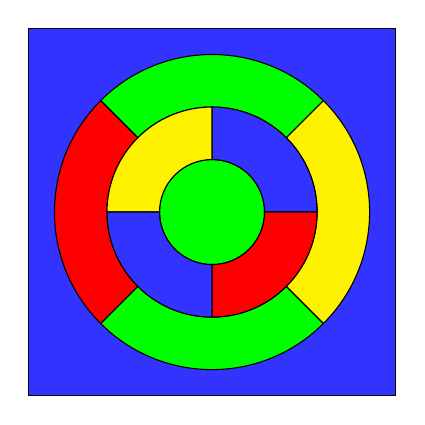
\begin{tikzpicture}[scale=.667]
\draw[fill=blue!80] (-3.5,-3.5) rectangle +(7,7);

\draw[fill=green] (0:1) 
  arc [start angle=0,  end angle=360, radius=1];

\draw[fill=green] (45:2) --
      (45:3)  arc[start angle=45,  end angle=135, radius=3] --
      (135:2) arc[start angle=135, end angle=45,  radius=2];
\draw[fill=green] (-45:2) --
      (-45:3)  arc[start angle=-45,  end angle=-135, radius=3] --
      (-135:2) arc[start angle=-135, end angle=-45,  radius=2];
\draw[fill=yellow] (45:2) --
      (45:3)  arc[start angle=45,  end angle=-45, radius=3] --
      (-45:2) arc[start angle=-45, end angle=45,  radius=2];
\draw[fill=red] (135:2) --
      (135:3)  arc[start angle=135,  end angle=225, radius=3] --
      (225:2) arc[start angle=225, end angle=135,  radius=2];

\draw[fill=blue!80] (0:1) --
      (0:2)  arc[start angle=0,  end angle=90, radius=2] --
      (90:1) arc[start angle=90, end angle=0,  radius=1];
\draw[fill=red] (0:1) --
      (0:2)  arc[start angle=0,  end angle=-90, radius=2] --
      (-90:1) arc[start angle=-90, end angle=0,  radius=1];
\draw[fill=yellow] (90:1) --
      (90:2)  arc[start angle=90,  end angle=180, radius=2] --
      (180:1) arc[start angle=180, end angle=90,  radius=1];
\draw[fill=blue!80] (180:1) --
      (180:2)  arc[start angle=180,  end angle=270, radius=2] --
      (270:1) arc[start angle=270, end angle=180,  radius=1];
\end{tikzpicture}
\caption{Vierfarbigkeit einer planaren Karte}\label{f.five-planar-map-four}
\end{minipage}
\end{figure}

\begin{definition}
Ein \emph{Graph} ist eine Menge von \emph{Scheitelpunkten} $V$ und eine Menge von \emph{Kanten} $E$, so dass jede Kante mit genau zwei Scheitelpunkten verbunden ist.

Ein \emph{planarer Graph} ist ein Graph, bei dem sich keine Kanten kreuzen. In einem planaren Graphen werden die von einer Menge von Kanten eingeschlossenen Bereiche \emph{Flächen} genannt.

Eine \emph{Farbgebung} eines planaren Graphen ist eine Zuordnung von Farben zu Knoten, so dass keine zwei Knoten der gleichen Farbe durch eine Kante verbunden sind.
\end{definition}

Planare Karten und planare Graphen sind dual und es ist bequem, Färbungsprobleme in Graphen statt in Karten zu untersuchen.

\begin{theorem}
Bei einer planaren Karte kann ein planarer Graph so konstruiert werden, dass es für jede Färbung der Regionen der Karte eine Färbung der Scheitelpunkte des Graphen gibt, und umgekehrt.
\end{theorem}

\begin{proof}
Konstruieren Sie einen Knoten für jede Region und konstruieren Sie eine Kante zwischen zwei Knoten, wenn und nur wenn die entsprechenden Regionen eine gemeinsame Grenze haben. 
\end{proof}

\begin{example}
Abbildung~\ref{f.five-planar-graph-map} zeigt die planare Karte aus Abb.~\ref{f.five-planar-map-four} und die mit den Regionen verbundenen Scheitelpunkte. Abbildung~\ref{f.five-planar-graph-graph} zeigt den planaren Graphen, der der Karte entspricht.
\end{example}

\begin{figure}[t]
\begin{minipage}{.45\textwidth}
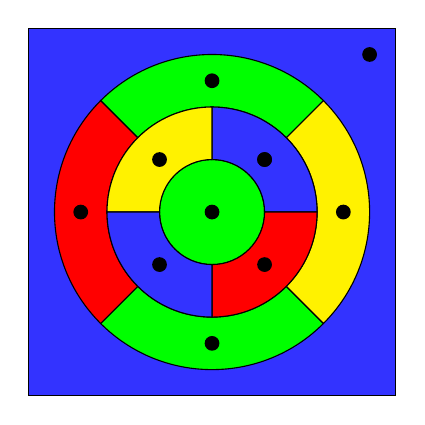
\begin{tikzpicture}[scale=.667]

\draw[fill=blue!80] (-3.5,-3.5) rectangle +(7,7);

\draw[fill=green] (0:1) 
  arc [start angle=0,  end angle=360, radius=1];

\draw[fill=green] (45:2) --
      (45:3)  arc[start angle=45,  end angle=135, radius=3] --
      (135:2) arc[start angle=135, end angle=45,  radius=2];
\draw[fill=green] (-45:2) --
      (-45:3)  arc[start angle=-45,  end angle=-135, radius=3] --
      (-135:2) arc[start angle=-135, end angle=-45,  radius=2];
\draw[fill=yellow] (45:2) --
      (45:3)  arc[start angle=45,  end angle=-45, radius=3] --
      (-45:2) arc[start angle=-45, end angle=45,  radius=2];
\draw[fill=red] (135:2) --
      (135:3)  arc[start angle=135,  end angle=225, radius=3] --
      (225:2) arc[start angle=225, end angle=135,  radius=2];

\draw[fill=blue!80] (0:1) --
      (0:2)  arc[start angle=0,  end angle=90, radius=2] --
      (90:1) arc[start angle=90, end angle=0,  radius=1];
\draw[fill=red] (0:1) --
      (0:2)  arc[start angle=0,  end angle=-90, radius=2] --
      (-90:1) arc[start angle=-90, end angle=0,  radius=1];
\draw[fill=yellow] (90:1) --
      (90:2)  arc[start angle=90,  end angle=180, radius=2] --
      (180:1) arc[start angle=180, end angle=90,  radius=1];
\draw[fill=blue!80] (180:1) --
      (180:2)  arc[start angle=180,  end angle=270, radius=2] --
      (270:1) arc[start angle=270, end angle=180,  radius=1];


\foreach \x/\y/\name in {
    0/0/O,
    3/3/Z,
    1/1/E,-1/1/F,-1/-1/G,1/-1/H,
    0/2.5/A,2.5/0/B,0/-2.5/C,-2.5/0/D,
    } {
  \fill (\x,\y) coordinate(\name) circle(4pt);
}
\end{tikzpicture}
\caption{Associating vertices with the regions of a planar map}\label{f.five-planar-graph-map}
\end{minipage}
\hfill
\begin{minipage}{.45\textwidth}
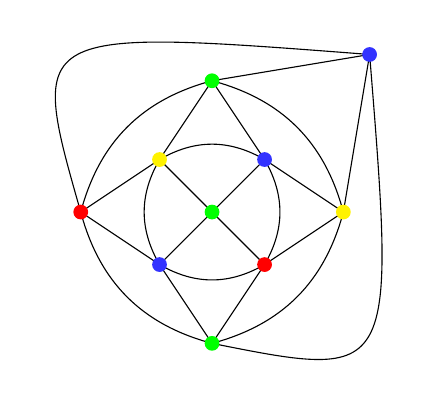
\begin{tikzpicture}[scale=.667]

\foreach \x/\y/\name in {
    0/0/O,
    3/3/Z,
    1/1/E,-1/1/F,-1/-1/G,1/-1/H,
    0/2.5/A,2.5/0/B,0/-2.5/C,-2.5/0/D,
    } {
  \coordinate(\name) at (\x,\y);
}

\draw (E) -- (O) -- (F);
\draw (G) -- (O) -- (H);
\draw (E) to [bend right=30] (F) to [bend right=30] (G) 
          to [bend right=30] (H) to [bend right=30] (E);
\draw (A) -- (E) -- (B) -- (H) -- (C) -- (G) -- (D) -- (F);
\draw (A) to [bend right=30] (D) to [bend right=30] (C) 
          to [bend right=30] (B) to [bend right=30] (A);

\draw (F) -- (A) -- (Z) -- (B);
\draw (C) .. controls (3.5,-3.2) .. (Z);
\draw (D) .. controls (-3.5,3.5) .. (Z);

\foreach \cl/\x/\y in {
    green/0cm/0cm,
    blue!80/3cm/3cm,
    blue!80/1cm/1cm,
    yellow/-1cm/1cm,
    blue!80/-1cm/-1cm,
    red/1cm/-1cm,
    green/0cm/2.5cm,
    yellow/2.5cm/0cm,
    green/0cm/-2.5cm,
    red/-2.5cm/0cm
    }
 \fill[\cl] (\x,\y) circle (4pt);
\end{tikzpicture}
\caption{Der planare Graph, der der planaren Karte entspricht}\label{f.five-planar-graph-graph}
\end{minipage}
\end{figure}

Wir können unsere Graphen weiter auf diejenigen beschränken, deren Flächen dreieckig sind.

\begin{definition}
Ein Graph ist \emph{dreieckig}, wenn alle seine Flächen durch drei Kanten begrenzt sind. Ein Graph kann \emph{trianguliert} werden, wenn Kanten hinzugefügt werden können, so dass der Graph dreieckig ist. Wir sagen auch, dass es eine \emph{Triangulation} des Graphen gibt.
\end{definition}

\begin{example}
Die Flächen des ebenen Graphen in Abb.~\ref{f.five-planar-graph-graph} sind dreieckig, da jede Fläche von drei Kanten begrenzt wird. Da die Kanten gekrümmt sind, handelt es sich bei den Flächen nicht um Dreiecke, sondern um Polygone, deren drei Kanten gerade Liniensegmente sind.
\end{example}

\begin{advanced}
\textbf{F\'{a}ry's Theorem} besagt, dass jeder dreieckige flächige Graph in einen äquivalenten flächigen Graph umgewandelt werden kann, dessen Kanten gerade Liniensegmente sind. Daher können die Beweise ohne Verlust an Allgemeinheit auf planare Graphen beschränkt werden, deren Flächen Dreiecke sind.
\end{advanced}

\begin{example}
Abb.~\ref{f.five-triangular-graph} (links) zeigt, dass ein Quadrat zweifarbig sein kann, aber wenn es trianguliert ist (Mitte), sind vier Farben notwendig. Unser Ziel ist es zu beweisen, dass \emph{all} Graphen $n$-farbig sein können für einige $n$. Wenn der triangulierte Graph $n$-farbig ist, dann ist es auch der ursprüngliche Graph, weil das Löschen der zusätzlichen Kanten die Färbung nicht ungültig macht (rechts).
\end{example}

\begin{figure}[ht]
\begin{center}
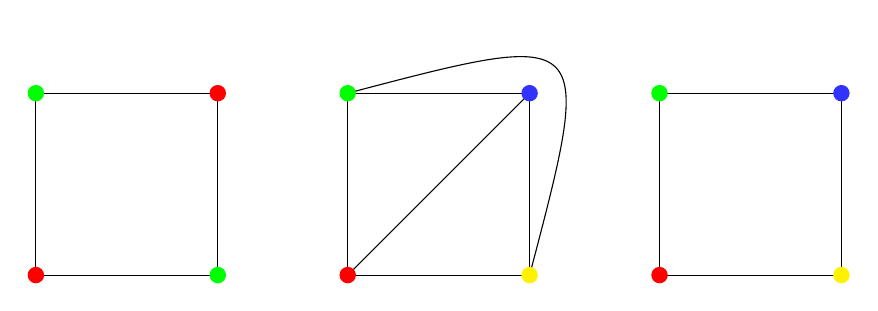
\begin{tikzpicture}[scale=.33]
\draw (-3.5,-3.5) rectangle +(7,7);
\fill[red] (-3.5,-3.5) circle(9pt);
\fill[green] (-3.5,3.5) circle(9pt);
\fill[green] (3.5,-3.5) circle(9pt);
\fill[red] (3.5,3.5) circle(9pt);
\begin{scope}[xshift=12cm]
\draw (-3.5,-3.5) -- (3.5,3.5);
\draw (-3.5,3.5) .. controls (6,6) .. (3.5,-3.5);
\draw (-3.5,-3.5) rectangle +(7,7);
\fill[red] (-3.5,-3.5) circle(9pt);
\fill[green] (-3.5,3.5) circle(9pt);
\fill[yellow] (3.5,-3.5) circle(9pt);
\fill[blue!80] (3.5,3.5) circle(9pt);
\end{scope}
\begin{scope}[xshift=24cm]
\draw (-3.5,-3.5) rectangle +(7,7);
\fill[red] (-3.5,-3.5) circle(9pt);
\fill[green] (-3.5,3.5) circle(9pt);
\fill[yellow] (3.5,-3.5) circle(9pt);
\fill[blue!80] (3.5,3.5) circle(9pt);
\end{scope}
\end{tikzpicture}
\end{center}
\caption{Färben eines triangulierten Graphen}\label{f.five-triangular-graph}
\end{figure}

\section{Eulersche Formel}\label{s.euler}

\begin{theorem}\label{thm.euler} Sei $G$ ein zusammenhängender planarer Graph mit $V$ Scheitelpunkten, $E$ Kanten und $F$ Flächen. Dann sei $V-E+F=2$.
\end{theorem}

\begin{proof}
Durch Induktion über die Anzahl der Kanten. Ist die Anzahl der Kanten im Graphen Null, so gibt es nur einen einzigen Scheitelpunkt und eine einzige Fläche, also $1-0+1=2$. Andernfalls gibt es mindestens eine Kante $e$ und sie verbindet zwei Scheitelpunkte $v_1,v_2$. Löschen Sie die Kante $e$.

\textit{Fall 1:}
Der Graph wird unzusammenhängend (Abb.~\ref{f.five-disconnected-removing}). Verschmelze $v_1$ mit $v_2$ (Abb.~\ref{f.five-disconnected-merge}). Der resultierende Graph $G'$ ist ein planarer zusammenhängender Graph und hat weniger Kanten als $G$, so dass nach der Induktionshypothese $(V-1)-(E-1)+F=2$, da auch die Anzahl der Scheitelpunkte um eins reduziert ist. Vereinfachend erhalten wir $V-E+F=2$ für $G$.
\begin{figure}[ht]
\begin{minipage}{.45\textwidth}
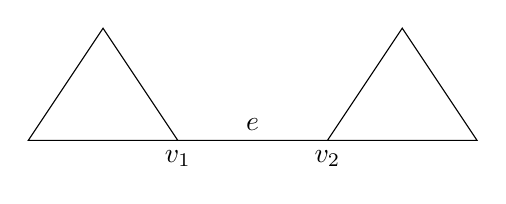
\begin{tikzpicture}[scale=.95]
\draw (2,0) -- (1,1.5) -- (0,0) -- (2,0) node[below] {$v_1$} -- node[above] {$e$} (4,0) node[below] {$v_2$} -- (6,0) -- (5,1.5) -- (4,0);
\end{tikzpicture}
\caption{Das Entfernen einer Kante unterbricht die Verbindung des Graphen}\label{f.five-disconnected-removing}
\end{minipage}
\hfill
\begin{minipage}{.45\textwidth}
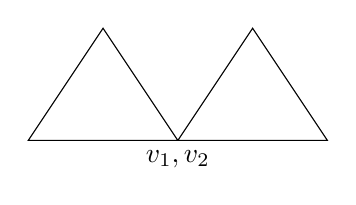
\begin{tikzpicture}[scale=.95]
\draw (2,0) -- (1,1.5) -- (0,0) -- (2,0) node[below] {$v_1,v_2$} -- (4,0) -- (3,1.5) -- (2,0);
\end{tikzpicture}
\caption{Verschmelzen von zwei Eckpunkten}\label{f.five-disconnected-merge}
\end{minipage}
\end{figure}

\textit{Fall 2:}
Der Graph bleibt verbunden (Abb.~\ref{f.five-connected-remains}). $G'$ hat weniger Kanten als $G$ (Abb.~\ref{f.five-connected-fewer}), so dass nach der Induktionshypothese $V-(E-1)+(F-1)=2$, da das Entfernen der Kante zwei Flächen zu einer verbindet. Vereinfachend erhalten wir $V-E+F=2$ für $G$.
\end{proof}

\begin{figure}[ht]
\begin{minipage}{.45\textwidth}
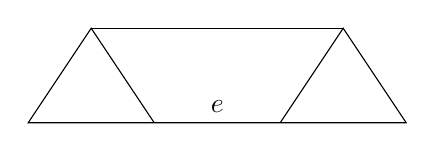
\begin{tikzpicture}[scale=.8]
\draw (2,0) -- (1,1.5) -- (0,0) -- (2,0) -- node[above] {$e$} (4,0) -- (6,0) -- (5,1.5) -- (4,0);
\draw (1,1.5) -- (5,1.5);
\end{tikzpicture}
\caption{Removing an edge does not disconnect the graph}\label{f.five-connected-remains}
\end{minipage}
\hfill
\begin{minipage}{.45\textwidth}
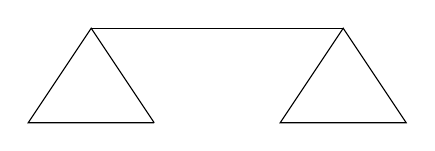
\begin{tikzpicture}[scale=.8]
\draw (2,0) -- (1,1.5) -- (0,0) -- (2,0);
\draw (4,0) -- (5,1.5) -- (6,0) -- cycle;
\draw (1,1.5) -- (5,1.5);
\end{tikzpicture}
\caption{Der Graph bleibt zusammenhängend und hat weniger Kanten}\label{f.five-connected-fewer}
\end{minipage}
\end{figure}

\begin{theorem}\label{thm.3v6}
Sei $G$ ein zusammenhängender, triangulierter, planarer Graph mit $E$ Kanten und $V$ Scheitelpunkten. Dann sei $E= 3V-6$.
\end{theorem}
\begin{proof}
Jede Fläche wird von drei Kanten begrenzt, also $E=3F/2$, wobei wir durch $2$ teilen, weil jede Kante zweimal gezählt wurde, einmal für jede Fläche, die sie begrenzt. Nach der Eulerschen Formel:
\begin{eqnarray*}
E&=&V+F-2\\
&=&V+2E/3-2\\
&=&3V-6\,.
\end{eqnarray*}
\end{proof}

\begin{example}
Der planare Graph in Abb.~\ref{f.five-planar-graph-graph} hat $10$ Eckpunkte und $3\cdot 10-6=24$ Kanten.
\end{example}

\begin{theorem}\label{thm.count}
Sei $G$ ein zusammenhängender planarer Graph. Dann sei $E\leq 3V-6$.
\end{theorem}

\begin{proof}
Triangulieren Sie $G$, um $G'$ zu erhalten. $E'= 3V'-6$ nach Thm.~\ref{thm.3v6}. Entfernen Sie nun Kanten aus $G'$, um $G$ zu erhalten. Die Anzahl der Scheitelpunkte ändert sich nicht, so dass $E'= 3V-6$ ist.
\end{proof}

\begin{example}
Der Graph in Abb.~\ref{f.five-fewer} hat $8$ Kanten und $6$ Scheitelpunkte und $8< 3\cdot 6 - 6= 12$.
Abbildung~\ref{f.five-upper-limit} zeigt einen triangulierten Graphen mit $6$ Scheitelpunkten und $3\cdot 6 - 6= 12$ Kanten.
\end{example}

\begin{figure}[t]
\begin{center}
\begin{minipage}{.4\textwidth}
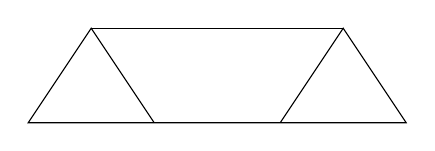
\begin{tikzpicture}[scale=.8]
\draw (2,0) -- (1,1.5) -- (0,0) -- (2,0) -- (4,0) -- (6,0) -- (5,1.5) -- (4,0);
\draw (1,1.5) -- (5,1.5);
\end{tikzpicture}
\caption{Weniger Kanten als die Obergrenze}\label{f.five-fewer}
\end{minipage}
\hfill
\begin{minipage}{.55\textwidth}
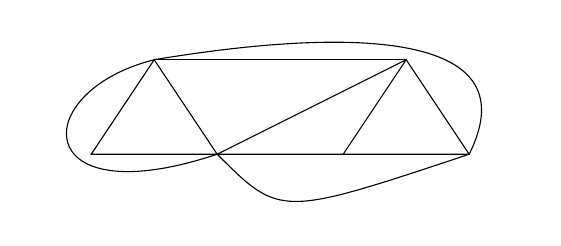
\begin{tikzpicture}[scale=.8]
\draw (2,0) -- (1,1.5) -- (0,0) -- (2,0) -- (4,0) -- (6,0) -- (5,1.5) -- (4,0);
\draw (1,1.5) -- (5,1.5);
\draw (2,0) -- (5,1.5);
\draw (2,0) .. controls (-1,-1) and (-1,1) .. (1,1.5);
\draw (2,0) .. controls (3,-1) .. (6,0) .. controls (7,2) and (4,2) .. (1,1.5);
\end{tikzpicture}
\caption{In einem triangulierten Graphen ist die Anzahl der Kanten maximal}\label{f.five-upper-limit}
\end{minipage}
\end{center}
\end{figure}

\section{Nicht-planare Diagramme}\label{s.nonplanar}

Lassen Sie uns einen kurzen Umweg machen, um zu zeigen, wie Thms.~\ref{thm.euler} und~\ref{thm.count} verwendet werden können, um zu beweisen, dass bestimmte Graphen nicht planar sind.

\begin{theorem}
$K_5$, der vollständige Graph mit fünf Scheitelpunkten, ist nicht planar (Fig.~\ref{f.five-k5}).
\end{theorem}

\begin{figure}[t]
\begin{minipage}{.45\textwidth}
\begin{tikzpicture}[scale=.8]
\node (pentagon) [minimum size=4cm,regular polygon,regular polygon sides=5] at (0,0) {};
\draw (pentagon.corner 1) -- (pentagon.corner 2);
\draw (pentagon.corner 2) -- (pentagon.corner 3);
\draw (pentagon.corner 3) -- (pentagon.corner 4);
\draw (pentagon.corner 4) -- (pentagon.corner 5);
\draw (pentagon.corner 5) -- (pentagon.corner 1);
\draw (pentagon.corner 1) -- (pentagon.corner 3);
\draw (pentagon.corner 1) -- (pentagon.corner 4);
\draw (pentagon.corner 2) -- (pentagon.corner 4);
\draw (pentagon.corner 2) -- (pentagon.corner 5);
\draw (pentagon.corner 3) -- (pentagon.corner 5);
\end{tikzpicture}
\caption{$K_5$ nicht planar ist}\label{f.five-k5}
\end{minipage}
\hfill
\begin{minipage}{.45\textwidth}
\begin{tikzpicture}[scale=.8]
\node (pentagon) [minimum size=4cm,regular polygon,regular polygon sides=5] at (0,0) {};
\draw (pentagon.corner 1) -- (pentagon.corner 2);
\draw (pentagon.corner 2) -- (pentagon.corner 3);
\draw (pentagon.corner 3) -- (pentagon.corner 4);
\draw (pentagon.corner 4) -- (pentagon.corner 5);
\draw (pentagon.corner 5) -- (pentagon.corner 1);
\draw (pentagon.corner 1) .. controls (-4,1) .. 
      (pentagon.corner 3);
\draw (pentagon.corner 1) .. controls (4,1) ..
      (pentagon.corner 4);
\draw (pentagon.corner 2) -- (pentagon.corner 4);
\draw (pentagon.corner 2) -- (pentagon.corner 5);
\draw (pentagon.corner 3) -- (pentagon.corner 5);
\draw[thick] (0,-.95) circle(5pt);
\end{tikzpicture}
\caption{Ein gescheiterter Versuch, $K_5$ als planar zu zeichnen}\label{f.five-k5-failed}
\end{minipage}
\end{figure}

\begin{proof}
Für $K_5$, $V=5$ und $E=10$. Nach Thm.~\ref{thm.count} muss die Anzahl der Kanten kleiner oder gleich $3\cdot 5 -6=9$ sein, also ist der Graph nicht planar.
\end{proof}

\begin{theorem}
$K_{3,3}$, der zweistufige Graph mit drei Eckpunkten auf jeder Seite, ist nicht planar (Abb.~\ref{f.five-k33}).
\end{theorem}

\begin{figure}[b]
\begin{minipage}{.45\textwidth}
\begin{center}
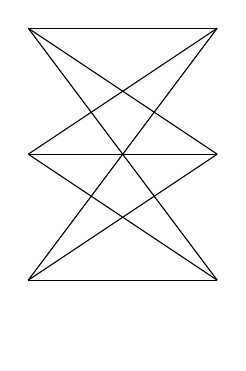
\begin{tikzpicture}[scale=.8]
\draw (0,0) -- (3,0);
\draw (0,2) -- (3,2);
\draw (0,4) -- (3,4);
\draw (0,0) -- (3,2);
\draw (0,2) -- (3,4);
\draw (0,4) -- (3,0);
\draw (0,0) -- (3,4);
\draw (0,2) -- (3,0);
\draw (0,4) -- (3,2);
\path (0,-1) -- (3,-1);
\end{tikzpicture}
\caption{$K_{3,3}$ nicht planar ist}\label{f.five-k33}
\end{center}
\end{minipage}
\hfill
\begin{minipage}{.45\textwidth}
\begin{center}
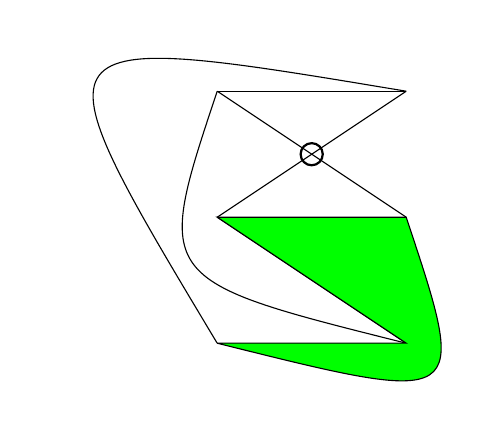
\begin{tikzpicture}[scale=.8]
\draw (0,4) -- (3,4);
\draw (0,2) -- (3,4);
\draw (0,4) .. controls (-1,1) .. (3,0);
\draw (0,0) .. controls (-3,5) .. (3,4);
\draw (0,2) -- (3,0);
\draw (0,4) -- (3,2);

\draw[fill=green] (0,0) -- (3,0) -- (3,0) -- (0,2)  -- (3,2) .. controls (4,-1) .. (0,0);
\draw[thick] (1.5,3) circle(5pt);
\end{tikzpicture}
\caption{Ein gescheiterter Versuch, $K_{3,3}$ als planar zu zeichnen}\label{f.five-k33-failed}
\end{center}
\end{minipage}
\end{figure}

\begin{proof}
$V=6$ und $E=9$. Nach Thm~\ref{thm.euler} ist, wenn $K_{3,3}$ planar ist, $F=E-V+2=9-6+2=5$. Aber jede Fläche wird durch vier Kanten begrenzt (Abb.~\ref{f.five-k33-failed}), also $E=4F/2=10\neq 9$.
\end{proof}

Im Jahr 1930 bewies Kazimierz Kuratowski eine Umkehrung dieser Theoreme: Wenn ein Graph nicht planar ist, enthält er (in einem bestimmten Sinne) $K_5$ oder $K_{3,3}$.

\section{Die Gradzahlen der Scheitelpunkte}\label{s.degrees}

\begin{definition}
$d(v)$, der \emph{Grad} des Scheitelpunkts $v$, ist die Anzahl der Kanten, die mit $v$.
\end{definition}

\begin{example}
Der Graph in Abb.~\ref{f.five-planar-graph-graph} enthält $8$ Scheitelpunkte, die den beiden Ringen entsprechen, und jeder Scheitelpunkt hat den Grad $5$. Der Scheitelpunkt, der der äußeren Fläche entspricht, hat den Grad $4$, ebenso der Scheitelpunkt, der der inneren Fläche entspricht. Daher
\[
\sum_{v\in V} d(v) = 5\cdot 8 + 4\cdot 2=48\,.
\]
Um die Gesamtzahl der Kanten zu erhalten, muss man $48$ durch $2$ teilen, da jede Kante zweimal gezählt wurde, einmal für jeden der Eckpunkte, mit denen sie verbunden ist.
\end{example}

Wenn wir das Argument verallgemeinern, erhalten wir:
\begin{theorem}\label{thm.degrees}
Sei $d_i$ für $i$ in $\{1,2,3,\ldots,k\}$ die Anzahl der Scheitelpunkte vom Grad $i$ in einem zusammenhängenden planaren Graphen $G$ mit $V$ Scheitelpunkten und $E$ Kanten, wobei $k$ der höchste Grad eines Scheitelpunktes in $V$ ist. Dann:
\[
\sum_{v\in V} d(v) =\sum_{i=1}^{k} i\cdot d_i=2E\,.
\]
\end{theorem}

\begin{theorem}\label{thm.degree5}
Sei $G$ ein zusammenhängender planarer Graph mit $E$ Kanten und $V$ Scheitelpunkten, und sei $d_i$ für $i$ in $\{1,2,3,\ldots,k\}$ die Anzahl der Scheitelpunkte vom Grad $i$, wobei $k$ der höchste Grad eines Scheitelpunktes in $V$ ist. Dann muss es einen Scheitelpunkt $v$ in $V$ geben, so dass $d(v) \leq 5$ ist.
\end{theorem}

\begin{proof}[1]
Wenn es $d_1$ Scheitelpunkte vom Grad $1$, $d_2$ Scheitelpunkte vom Grad $2$, \ldots, $d_k$ Scheitelpunkte vom Grad $k$ gibt, dann $V=\sum_{i=1}^{k}d_i$.  Aus Thms.~\ref{thm.count} und \ref{thm.degrees}:
\[
\sum_{i=1}^{k} i\cdot d_i=2E\leq 2(3V-6) = 6V-12=6\sum_{i=1}^{k} d_i -12\,.
\]
Deshalb:
\begin{eqnarray*}
\sum_{i=1}^{k} i\cdot d_i &\leq& 6\sum_{i=1}^{k} d_i -12\\
\sum_{i=1}^{k} (6-i)d_i&\geq& 12\,.
\end{eqnarray*}
Da $12>0$ und alle $d_i$ positiv sind, ist für mindestens ein $i$, $6-i>0$ und für dieses $i$, $i<6$.
\end{proof}

\begin{proof}[2]
Berechnen wir den \emph{durchschnittlichen} Grad der Scheitelpunkte, der die Summe der Grade geteilt durch die Anzahl der Scheitelpunkte ist:
\[
d_{\textit{\footnotesize avg}}=\frac{\sum_{i=1}^{k} i\cdot d_i}{V}\,.
\]
Aber die Summe der Grade ist das Doppelte der Anzahl der Kanten, was nach Thm.~\ref{thm.count} ergibt:
\[
d_{\textit{\footnotesize avg}}=\frac{2E}{V}\leq \frac{6V-12}{V}=6-\frac{6}{V}<6\,.
\]
Wenn der Durchschnitt kleiner als sechs ist, muss es einen Scheitelpunkt vom Grad kleiner als sechs geben.
\end{proof}

\begin{example}
In Abb.~\ref{f.five-planar-graph-graph} ist die Summe der Grade $8\cdot 5 + 2\cdot 4=48$. Es gibt $10$ Scheitelpunkte, also ist der durchschnittliche Grad $48/10=4.8$ und es muss einen Scheitelpunkt mit dem Grad $4$ oder weniger geben.
\end{example}

\section{Das Sechs-Farben-Theorem}\label{s.six-color}

\begin{theorem}\label{thm.sixcolor}
Jeder planare Graph $G$ kann sechsfarbig sein.
\end{theorem}
\begin{proof}
Durch Induktion auf die Anzahl der Scheitelpunkte. Wenn $G$ sechs Scheitelpunkte oder weniger hat, genügen sechs Farben.
Für den Induktionsschritt hat $G$ nach Thm.~\ref{thm.degree5} einen Scheitelpunkt $v$ mit Grad $5$ oder weniger. Löschen Sie den Knoten $v$, um den Graphen $G'$ zu erhalten. Nach der Induktionshypothese kann $G'$ sechsfarbig sein, aber $v$ hat höchstens $5$ Nachbarn und es werden höchstens $5$ Farben verwendet, um sie zu färben (Abb.~\ref{f.five-six-five}), also kann $v$ mit der sechsten Farbe gefärbt werden (Abb.~\ref{f.five-six-six}).
\end{proof}

\begin{figure}[hbt]
\begin{minipage}{.45\textwidth}
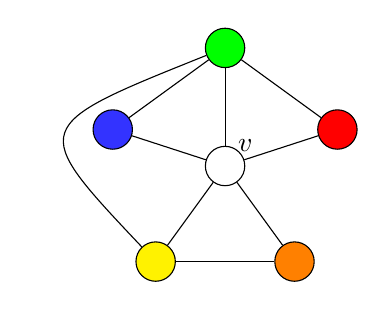
\begin{tikzpicture}[scale=.5,minimum size=5mm,inner sep=0pt]
\foreach \name/\color/\theta in
    {A/red/18,B/green/90,C/blue!80/162,D/yellow/234,E/orange/306}
  \node[circle,draw,fill=\color] (\name) at (\theta:3) {};
\node[circle,draw] (O) at (0,0) {};
\node[above right] at (O) {$v$};
\foreach \name in {A,B,C,D,E}
  \draw (O) -- (\name);
\foreach \i/\j in {A/B,B/C,D/E}
  \draw (\i) -- (\j);
\draw (B) .. controls (-5,1) .. (D);
\end{tikzpicture}
\caption{Fünf Farben reichen aus, um die Nachbarn von $v$}\label{f.five-six-five}
\end{minipage}
\hfill
\begin{minipage}{.45\textwidth}
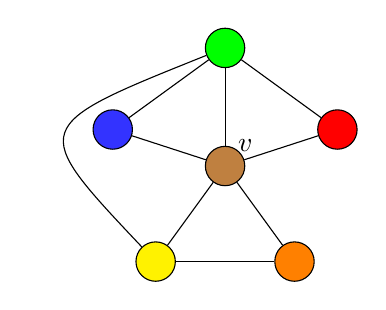
\begin{tikzpicture}[scale=.5,minimum size=5mm,inner sep=0pt]
\foreach \name/\color/\theta in
    {A/red/18,B/green/90,C/blue!80/162,D/yellow/234,E/orange/306}
  \node[circle,draw,fill=\color] (\name) at (\theta:3) {};
\node[circle,draw,fill=brown] (O) at (0,0) {};
\node[above right] at (O) {$v$};
\foreach \name in {A,B,C,D,E}
  \draw (O) -- (\name);
\foreach \i/\j in {A/B,B/C,D/E}
  \draw (\i) -- (\j);
\draw (B) .. controls (-5,1) .. (D);
\end{tikzpicture}
\caption{Färbe $v$ mit der sechsten Farbe}\label{f.five-six-six}
\end{minipage}
\end{figure}

\section{Das Fünf-Farben-Theorem}\label{s.five-color}

\begin{definition}
Sei $G$ ein farbiger planarer Graph. Eine \emph{(Kempe)-Kette} $G'$ ist ein maximaler, zweifarbiger, zusammenhängender Untergraph von $G$.
\end{definition}
 
\begin{theorem}\label{thm.fivecolor}
Jeder planare Graph $G$ kann fünffarbig sein.
\end{theorem}

\begin{proof}
Durch Induktion auf die Anzahl der Scheitelpunkte. Wenn $G$ fünf Scheitelpunkte oder weniger hat, genügen fünf Farben.
Für den Induktionsschritt hat $G$ nach Thm.~\ref{thm.degree5} einen Scheitelpunkt $v$ mit Grad $5$ oder weniger. Löschen Sie $v$, um $G'$ zu erhalten. Nach der Induktionshypothese kann $G'$ fünffarbig sein. In $G$ kann $v$ mit der fünften Farbe gefärbt werden, wenn der Grad von $v$ kleiner als $5$ ist, oder wenn $v_1,\ldots,v_5$, die Nachbarn von $v$, mit vier oder weniger Farben gefärbt sind.
Andernfalls werden $v_1,\ldots,v_5$ in $G'$ mit verschiedenen Farben gefärbt (Abb.~\ref{f.five-color-proof}, oben).

\begin{figure}
\begin{center}
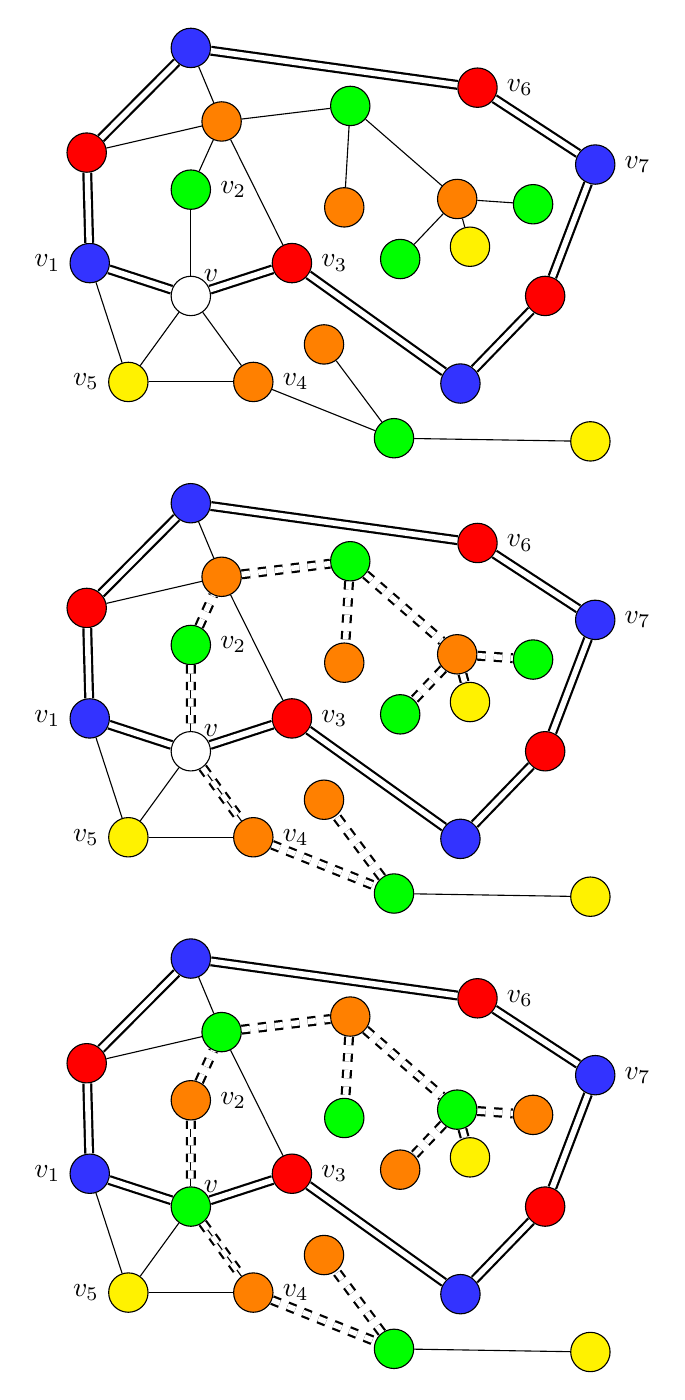
\begin{tikzpicture}[scale=.45,minimum size=5mm,inner sep=0pt]
\foreach \name/\color/\theta in
    {A/red/18,B/green/90,C/blue!80/162,D/yellow/234,E/orange/306}
  \node[circle,draw,fill=\color] (\name) at (\theta:3) {};
\node[circle,draw] (O) at (0,0) {};
\node[above right] at (O) {$v$};

\node[right,xshift=8pt] at (A) {$v_3$};
\node[right,xshift=8pt] at (B) {$v_2$};
\node[left,,xshift=-8pt] at (C) {$v_1$};
\node[left,,xshift=-8pt] at (D) {$v_5$};
\node[right,xshift=8pt] at (E) {$v_4$};

\foreach \name in {A,B,C,D,E}
  \draw (O) -- (\name);
  
\node[circle,draw,fill=red]  (X1) at (126:5) {};
\node[circle,draw,fill=blue!80] (X2) at (90:7)  {};
\node[circle,draw,fill=red]  (X3) at (36:10) {};
\node[right,xshift=8pt] at (X3) {$v_6$};
\node[circle,draw,fill=blue!80] (X4) at (18:12) {};
\node[right,xshift=8pt] at (X4) {$v_7$};
\node[circle,draw,fill=red]  (X5) at (0:10) {};
\node[circle,draw,fill=blue!80] (X6) at (-18:8) {};
\draw[thick,double distance=2pt] (C)  -- (X1);
\draw[thick,double distance=2pt] (X1) -- (X2);
\draw[thick,double distance=2pt] (X2) -- (X3);
\draw[thick,double distance=2pt] (X3) -- (X4);
\draw[thick,double distance=2pt] (X4) -- (X5);
\draw[thick,double distance=2pt] (X5) -- (X6);
\draw[thick,double distance=2pt] (X6) -- (A);
\draw[thick,double distance=2pt] (A) -- (O) -- (C);

\node[circle,draw,fill=orange]  (Y1)  at (80:5) {};
\node[circle,draw,fill=green]   (Y2)  at (50:7)  {};
\node[circle,draw,fill=orange]  (Y3A) at (20:8) {};
\node[circle,draw,fill=orange]  (Y3B) at (30:5) {};
\node[circle,draw,fill=green]   (Y4A) at (10:6) {};
\node[circle,draw,fill=yellow]  (Y4B) at (10:8) {};
\node[circle,draw,fill=green]   (Y4C) at (15:10) {};
\node[circle,draw,fill=green]   (Y5)  at (-35:7) {};
\node[circle,draw,fill=yellow]  (Y6A) at (-20:12) {};
\node[circle,draw,fill=orange]  (Y6B) at (-20:4) {};
\draw (B)  -- (Y1);
\draw (Y1) -- (Y2);
\draw (Y2) -- (Y3A);
\draw (Y2) -- (Y3B);
\draw (Y3A) -- (Y4A);
\draw (Y3A) -- (Y4B);
\draw (Y3A) -- (Y4C);
\draw (E)  -- (Y5);
\draw (Y5) -- (Y6A);
\draw (Y5) -- (Y6B);
\draw (A) -- (Y1);
\draw (X2) -- (Y1);
\draw (X1) -- (Y1);
\draw (D) -- (E);
\draw (D) -- (C);

\begin{scope}[yshift=-12.85cm]
\foreach \name/\color/\theta in
    {A/red/18,B/green/90,C/blue!80/162,D/yellow/234,E/orange/306}
  \node[circle,draw,fill=\color] (\name) at (\theta:3) {};
\node[circle,draw] (O) at (0,0) {};
\node[above right] at (O) {$v$};

\node[right,xshift=8pt] at (A) {$v_3$};
\node[right,xshift=8pt] at (B) {$v_2$};
\node[left,,xshift=-8pt] at (C) {$v_1$};
\node[left,,xshift=-8pt] at (D) {$v_5$};
\node[right,xshift=8pt] at (E) {$v_4$};

\foreach \name in {A,B,C,D,E}
  \draw (O) -- (\name);
  
\node[circle,draw,fill=red]  (X1) at (126:5) {};
\node[circle,draw,fill=blue!80] (X2) at (90:7)  {};
\node[circle,draw,fill=red]  (X3) at (36:10) {};
\node[circle,draw,fill=blue!80] (X4) at (18:12) {};
\node[circle,draw,fill=red]  (X5) at (0:10) {};
\node[circle,draw,fill=blue!80] (X6) at (-18:8) {};

\draw[thick,double distance=2pt] (C)  -- (X1);
\draw[thick,double distance=2pt] (X1) -- (X2);
\draw[thick,double distance=2pt] (X2) -- (X3);
\draw[thick,double distance=2pt] (X3) -- (X4);
\draw[thick,double distance=2pt] (X4) -- (X5);
\draw[thick,double distance=2pt] (X5) -- (X6);
\draw[thick,double distance=2pt] (X6) -- (A);
\draw[thick,double distance=2pt] (A) -- (O) -- (C);

\node[circle,draw,fill=orange]  (Y1)  at (80:5) {};
\node[circle,draw,fill=green]   (Y2)  at (50:7)  {};
\node[circle,draw,fill=orange]  (Y3A) at (20:8) {};
\node[circle,draw,fill=orange]  (Y3B) at (30:5) {};
\node[circle,draw,fill=green]   (Y4A) at (10:6) {};
\node[circle,draw,fill=yellow]   (Y4B) at (10:8) {};
\node[circle,draw,fill=green]   (Y4C) at (15:10) {};
\node[circle,draw,fill=green]   (Y5)  at (-35:7) {};
\node[circle,draw,fill=yellow]  (Y6A) at (-20:12) {};
\node[circle,draw,fill=orange]  (Y6B) at (-20:4) {};
\draw[thick,dashed,double distance=2pt] (B)  -- (O) -- (E);
\draw[thick,dashed,double distance=2pt] (B)  -- (Y1);
\draw[thick,dashed,double distance=2pt] (Y1) -- (Y2);
\draw[thick,dashed,double distance=2pt] (Y2) -- (Y3A);
\draw[thick,dashed,double distance=2pt] (Y2) -- (Y3B);
\draw[thick,dashed,double distance=2pt] (Y3A) -- (Y4A);
\draw[thick,dashed,double distance=2pt] (Y3A) -- (Y4B);
\draw[thick,dashed,double distance=2pt] (Y3A) -- (Y4C);
\draw[thick,dashed,double distance=2pt] (E)  -- (Y5);
\draw[thick,dashed,double distance=2pt] (Y5) -- (Y6B);
\draw (Y5) -- (Y6A);
\draw (A) -- (Y1);
\draw (X2) -- (Y1);
\draw (X1) -- (Y1);
\draw (D) -- (E);
\draw (D) -- (C);
\node[right,xshift=8pt] at (X3) {$v_6$};
\node[right,xshift=8pt] at (X4) {$v_7$};
\end{scope}

\begin{scope}[yshift=-25.7cm]
\foreach \name/\color/\theta in
    {A/red/18,B/orange/90,C/blue!80/162,D/yellow/234,E/orange/306}
  \node[circle,draw,fill=\color] (\name) at (\theta:3) {};
\node[circle,draw,fill=green] (O) at (0,0) {};
\node[above right] at (O) {$v$};

\node[right,xshift=8pt] at (A) {$v_3$};
\node[right,xshift=8pt] at (B) {$v_2$};
\node[left,,xshift=-8pt] at (C) {$v_1$};
\node[left,,xshift=-8pt] at (D) {$v_5$};
\node[right,xshift=8pt] at (E) {$v_4$};

\foreach \name in {A,B,C,D,E}
  \draw (O) -- (\name);
  
\node[circle,draw,fill=red]  (X1) at (126:5) {};
\node[circle,draw,fill=blue!80] (X2) at (90:7)  {};
\node[circle,draw,fill=red]  (X3) at (36:10) {};
\node[circle,draw,fill=blue!80] (X4) at (18:12) {};
\node[circle,draw,fill=red]  (X5) at (0:10) {};
\node[circle,draw,fill=blue!80] (X6) at (-18:8) {};

\draw[thick,double distance=2pt] (C)  -- (X1);
\draw[thick,double distance=2pt] (X1) -- (X2);
\draw[thick,double distance=2pt] (X2) -- (X3);
\draw[thick,double distance=2pt] (X3) -- (X4);
\draw[thick,double distance=2pt] (X4) -- (X5);
\draw[thick,double distance=2pt] (X5) -- (X6);
\draw[thick,double distance=2pt] (X6) -- (A);
\draw[thick,double distance=2pt] (A) -- (O) -- (C);

\node[circle,draw,fill=green]  (Y1)  at (80:5) {};
\node[circle,draw,fill=orange]   (Y2)  at (50:7)  {};
\node[circle,draw,fill=green]  (Y3A) at (20:8) {};
\node[circle,draw,fill=green]  (Y3B) at (30:5) {};
\node[circle,draw,fill=orange]   (Y4A) at (10:6) {};
\node[circle,draw,fill=yellow]   (Y4B) at (10:8) {};
\node[circle,draw,fill=orange]   (Y4C) at (15:10) {};
\node[circle,draw,fill=green]   (Y5)  at (-35:7) {};
\node[circle,draw,fill=yellow]  (Y6A) at (-20:12) {};
\node[circle,draw,fill=orange]  (Y6B) at (-20:4) {};

\draw[thick,dashed,double distance=2pt] (B)  -- (O) -- (E);
\draw[thick,dashed,double distance=2pt] (B)  -- (Y1);
\draw[thick,dashed,double distance=2pt] (Y1) -- (Y2);
\draw[thick,dashed,double distance=2pt] (Y2) -- (Y3A);
\draw[thick,dashed,double distance=2pt] (Y2) -- (Y3B);
\draw[thick,dashed,double distance=2pt] (Y3A) -- (Y4A);
\draw[thick,dashed,double distance=2pt] (Y3A) -- (Y4B);
\draw[thick,dashed,double distance=2pt] (Y3A) -- (Y4C);
\draw[thick,dashed,double distance=2pt] (E)  -- (Y5);
\draw[thick,dashed,double distance=2pt] (Y5) -- (Y6B);


\draw (Y5) -- (Y6A);
\draw (A) -- (Y1);
\draw (X2) -- (Y1);
\draw (X1) -- (Y1);
\draw (D) -- (E);
\draw (D) -- (C);
\node[right,xshift=8pt] at (X3) {$v_6$};
\node[right,xshift=8pt] at (X4) {$v_7$};
\end{scope}
\end{tikzpicture}
\end{center}
\caption{Beweis des Fünf-Farben-Satzes}\label{f.five-color-proof}
\end{figure}

Betrachten wir den blau gefärbten Scheitelpunkt $v_1$ und den rot gefärbten Scheitelpunkt $v_3$. Wenn $v_1,v_3$ nicht durch einen blau-roten Pfad verbunden sind (z.B. wenn die Kante $\overline{v_6v_7}$ nicht existiert), können wir die Farben entlang des Pfades von $v_1$ nach $v_6$ vertauschen und $v$ blau färben. Andernfalls betrachten wir die blau-rote Kette, die $v_1,v_3$ enthält. Durch Addition von $v$ und den Kanten $\overline{vv_1},\overline{vv_3}$ erhalten wir einen geschlossenen Pfad $P$ (Doppellinie), der die Ebene in einen ``inneren'' Bereich und einen ``äußeren'' Bereich teilt (Abb.~\ref{f.five-color-proof}, Mitte)

Betrachten Sie $v_2$, das grün gefärbt ist, und $v_4$, das orange gefärbt ist. Diese Scheitelpunkte können nicht in einer einzigen grün-orangen Kette enthalten sein, weil $v_2$ innerhalb von $P$ und $v_4$ außerhalb von $P$ liegt, so dass jeder Pfad, der sie verbindet, $P$ durchqueren muss, was der Annahme widerspricht, dass der Graph planar ist. Daher müssen sie in zwei \emph{unverbundenen} grün-orangenen Ketten enthalten sein (doppelt gestrichelte Linie, in Abb.~\ref{f.five-color-proof}, Mitte).
Vertauscht man die Farben der Kette, die $v_2$ enthält, so kann $v$ grün gefärbt werden und man erhält eine Fünffärbung von $G$ (Abb.~\ref{f.five-color-proof}, unten).
\end{proof}

\begin{advanced}
Die Aussage, dass ein kontinuierlicher Pfad von der \emph{innen} einer geschlossenen kontinuierlichen Kurve $P$ zur \emph{außen} von $P$ $P$ schneiden muss, ist der \textbf{Jordan Curve Theorem}. Der Satz ist intuitiv offensichtlich, aber schwer zu beweisen.
\end{advanced}

\section{Kempes falscher Beweis des Vier-Farben-Satzes}\label{s.kempe}

\begin{theorem}\label{thm.fourcolor}
Jeder planare Graph $G$ kann vierfarbig sein.
\end{theorem}

\begin{proof}[Falsch] Der Grundfall der Induktion und der größte Teil des Beweises ist derselbe wie der des Fünf-Farben-Satzes. Der neue Fall, der betrachtet werden muss, ist ein Scheitelpunkt $v$ mit fünf Nachbarn, der nach der Induktionshypothese mit vier Farben gefärbt werden kann, nachdem $v$ entfernt wurde.

In Abb.~\ref{f.five-kempe1} gibt es zwei blau gefärbte Knoten $v_2,v_5$. Betrachten Sie die blau-grüne Kette mit $v_2$ und die blau-gelbe Kette mit $v_5$. Die blau-grüne Kette ist in dem geschlossenen Pfad enthalten, der durch die rot-gelbe Kette, die $v_1,v_3$ enthält, definiert ist (doppelte Linie), und die blau-gelbe Kette ist in dem geschlossenen Pfad enthalten, der durch die rot-grüne Kette, die $v_1,v_4$ enthält, definiert ist (doppelt gestrichelte Linie).

Tauschen Sie die Farben der blau-grünen Kette und der blau-gelben Kette (Abb.~\ref{f.five-kempe1-exchange}). Das Ergebnis ist, dass die Nachbarn von $v$ mit den drei Farben Rot, Grün und Gelb eingefärbt werden, so dass Blau als Farbe für $v$ frei bleibt.
\end{proof}

\begin{figure}[ht]
\begin{minipage}{.45\textwidth}
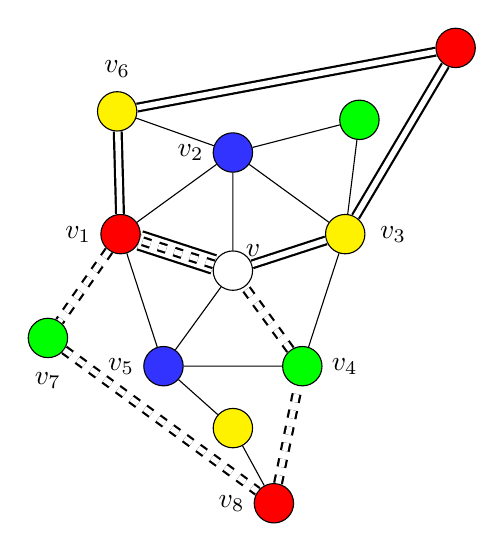
\begin{tikzpicture}[scale=.5,minimum size=5mm,inner sep=0pt]

% Draw center node and adjacent nodes
\foreach \name/\color/\theta in
    {A/yellow/18,B/blue!80/90,C/red/162,D/blue!80/234,E/green/306}
  \node[circle,draw,fill=\color] (\name) at (\theta:3) {};
\node[circle,draw] (O) at (0,0) {};
\node[above right]     at (O) {$v$};

\node[right,xshift=10pt] at (A) {$v_3$};
\node[left,xshift=-8pt]  at (B) {$v_2$};
\node[left,xshift=-8pt]  at (C) {$v_1$};
\node[left,xshift=-8pt]  at (D) {$v_5$};
\node[right,xshift=8pt]  at (E) {$v_4$};

% Draw red-yellow path
\node[circle,draw,fill=yellow]  (X1) at (126:5) {};
\node[circle,draw,fill=red] (X2) at (45:8)  {};

\draw[thick,double distance=2pt] 
  (C) -- (X1) -- (X2) -- (A) -- (O);
\draw[thick,double distance=6pt] (O) -- (C);

% Draw blue-green nodes within red-yellow path
\node[circle,draw,fill=green] (Y1)  at (50:5) {};

% Draw red-green path
\node[circle,draw,fill=green] (Z1)  at (-160:5) {};
\node[circle,draw,fill=red]   (Z2)  at (-80:6)  {};

\draw[thick,dashed,double distance=2pt] 
  (O) -- (C) -- (Z1) -- (Z2) -- (E) -- (O);

% Draw blue-yellow nodes within red-green path
\node[circle,draw,fill=yellow]   (U1)  at (-90:4)  {};

% Connect adjacent nodes not in paths
\draw (X1) -- (B) -- (Y1) -- (A) -- (B) -- 
      (C) -- (D) -- (E) -- (A);
\draw (Z2) -- (U1) -- (D) -- (O) -- (B);
\node[above,yshift=8pt] at (X1) {$v_6$};
\node[below,yshift=-8pt] at (Z1) {$v_7$};
\node[left,xshift=-8pt] at (Z2) {$v_8$};
\end{tikzpicture}
\caption{Blaugrüne und blau-gelbe Kempe-Ketten}\label{f.five-kempe1}
\end{minipage}
\hfill
\begin{minipage}{.45\textwidth}
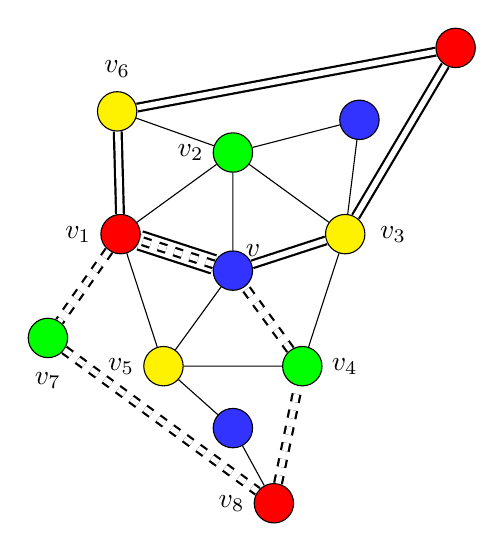
\begin{tikzpicture}[scale=.5,minimum size=5mm,inner sep=0pt]

% Draw center node and adjacent nodes
\foreach \name/\color/\theta in
    {A/yellow/18,B/green/90,C/red/162,D/yellow/234,E/green/306}
  \node[circle,draw,fill=\color] (\name) at (\theta:3) {};
\node[circle,draw,fill=blue!80] (O) at (0,0) {};
\node[above right]     at (O) {$v$};

\node[right,xshift=10pt] at (A) {$v_3$};
\node[left,xshift=-8pt]  at (B) {$v_2$};
\node[left,xshift=-8pt]  at (C) {$v_1$};
\node[left,xshift=-8pt]  at (D) {$v_5$};
\node[right,xshift=8pt]  at (E) {$v_4$};

% Draw red-yellow path
\node[circle,draw,fill=yellow]  (X1) at (126:5) {};
\node[circle,draw,fill=red] (X2) at (45:8)  {};

\draw[thick,double distance=2pt] 
  (C) -- (X1) -- (X2) -- (A) -- (O);
\draw[thick,double distance=6pt] (O) -- (C);

% Draw blue-green nodes within red-yellow path
\node[circle,draw,fill=blue!80] (Y1)  at (50:5) {};

% Draw red-green path
\node[circle,draw,fill=green] (Z1)  at (-160:5) {};
\node[circle,draw,fill=red]   (Z2)  at (-80:6)  {};

\draw[thick,dashed,double distance=2pt] 
  (O) -- (C) -- (Z1) -- (Z2) -- (E) -- (O);

% Draw blue-yellow nodes within red-green path
\node[circle,draw,fill=blue!80]   (U1)  at (-90:4)  {};

% Connect adjacent nodes not in paths
\draw (X1) -- (B) -- (Y1) -- (A) -- (B) -- 
      (C) -- (D) -- (E) -- (A);
\draw (Z2) -- (U1) -- (D) -- (O) -- (B);
\node[above,yshift=8pt] at (X1) {$v_6$};
\node[below,yshift=-8pt] at (Z1) {$v_7$};
\node[left,xshift=-8pt] at (Z2) {$v_8$};
\end{tikzpicture}
\caption{Tauschen Sie die Farben der beiden Kempe-Ketten}\label{f.five-kempe1-exchange}
\end{minipage}
\end{figure}

Heawood stellte fest, dass die geschlossenen Pfade, die durch die rot-gelbe Kette und die rot-grüne Kette definiert sind, rote Scheitelpunkte teilen können ($v_1,v_8$ in Abb.~\ref{f.five-kempe2}). Wenn die Farben in den blau-grünen und blau-gelben Ketten ausgetauscht werden, ist es möglich, dass die blauen Knoten $v_6,v_7$ verbunden sind (Abb.~\ref{f.five-kempe2-share}) und die Färbung nicht mehr korrekt ist.

\begin{figure}[ht]
\begin{minipage}{.45\textwidth}
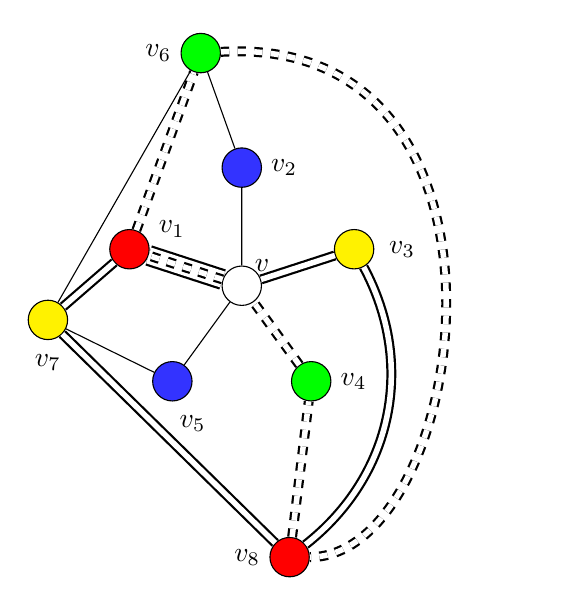
\begin{tikzpicture}[scale=.5,minimum size=5mm,inner sep=0pt]

% Draw center node and adjacent nodes
\foreach \name/\color/\theta in
    {A/yellow/18,B/blue!80/90,C/red/162,D/blue!80/234,E/green/306}
  \node[circle,draw,fill=\color] (\name) at (\theta:3) {};
\node[circle,draw] (O) at (0,0) {};
\node[above right]     at (O) {$v$};

\node[right,xshift=10pt] at (A) {$v_3$};
\node[right,xshift=8pt]  at (B) {$v_2$};
\node[above right,xshift=8pt]  at (C) {$v_1$};
\node[below right,yshift=-8pt] at (D) {$v_5$};
\node[right,xshift=8pt]  at (E) {$v_4$};

% Draw red-yellow path
\node[circle,draw,fill=yellow] (X1) at (-170:5) {};
\node[circle,draw,fill=red]    (X2) at (-80:7)  {};

\draw[thick,double distance=2pt] (A) -- (O);
\draw[thick,double distance=6pt] (O) -- (C);
\draw[thick,double distance=2pt] (C) --(X1) -- (X2);
\draw[thick,double distance=2pt,bend right=40] (X2) to (A);

% Draw red-green path
\node[circle,draw,fill=green] (Y1) at (100:6)  {};

\draw[dashed,thick,double distance=2pt] (O) -- (C) -- (Y1);
\draw[dashed,thick,double distance=2pt] 
  (Y1) .. controls (40:10) and (-50:9) .. (X2);
\draw[dashed,thick,double distance=2pt] (X2) -- (E) -- (O);

% Draw adjacent nodes
\draw (X1) -- (D) -- (O) -- (B) -- (Y1) -- (X1);
\node[left,xshift=-8pt] at (Y1) {$v_6$};
\node[below,yshift=-8pt] at (X1) {$v_7$};
\node[left,xshift=-8pt] at (X2) {$v_8$};
\end{tikzpicture}
\caption{Rot-gelbe und rot-grüne Ketten teilen sich rote Scheitelpunkte}\label{f.five-kempe2}
\end{minipage}
\hfill
\begin{minipage}{.45\textwidth}
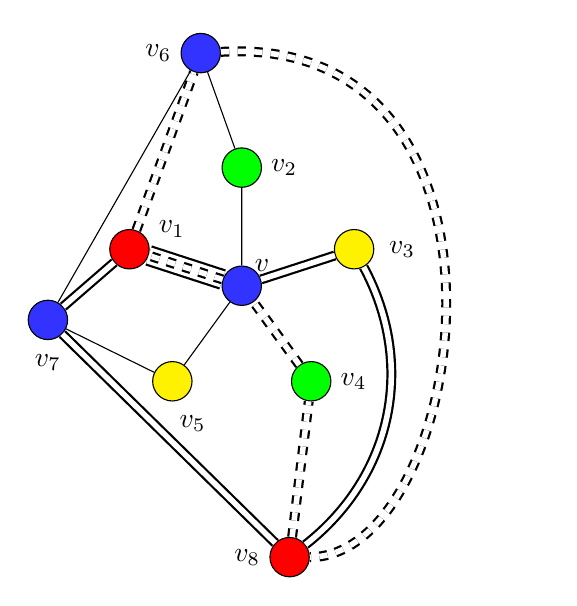
\begin{tikzpicture}[scale=.5,minimum size=5mm,inner sep=0pt]

% Draw center node and adjacent nodes
\foreach \name/\color/\theta in
    {A/yellow/18,B/green/90,C/red/162,D/yellow/234,E/green/306}
  \node[circle,draw,fill=\color] (\name) at (\theta:3) {};
\node[circle,draw,fill=blue!80] (O) at (0,0) {};
\node[above right]     at (O) {$v$};

\node[right,xshift=10pt] at (A) {$v_3$};
\node[right,xshift=8pt]  at (B) {$v_2$};
\node[above right,xshift=8pt]  at (C) {$v_1$};
\node[below right,yshift=-8pt] at (D) {$v_5$};
\node[right,xshift=8pt]  at (E) {$v_4$};

% Draw red-yellow path
\node[circle,draw,fill=blue!80] (X1) at (-170:5) {};
\node[circle,draw,fill=red]  (X2) at (-80:7)  {};

\draw[thick,double distance=2pt] (A) -- (O);
\draw[thick,double distance=6pt] (O) -- (C);
\draw[thick,double distance=2pt] (C) --(X1) -- (X2);
\draw[thick,double distance=2pt,bend right=40] (X2) to (A);

% Draw red-green path
\node[circle,draw,fill=blue!80] (Y1) at (100:6)  {};

\draw[dashed,thick,double distance=2pt] (O) -- (C) -- (Y1);
\draw[dashed,thick,double distance=2pt] 
  (Y1) .. controls (40:10) and (-50:9) .. (X2);
\draw[dashed,thick,double distance=2pt] (X2) -- (E) -- (O);

% Draw adjacent nodes
\draw (X1) -- (D) -- (O) -- (B) -- (Y1) -- (X1);
\node[left,xshift=-8pt] at (Y1) {$v_6$};
\node[below,yshift=-8pt] at (X1) {$v_7$};
\node[left,xshift=-8pt] at (X2) {$v_8$};
\end{tikzpicture}
\caption{Durch den Austausch der Farben werden die blauen Eckpunkte miteinander verbunden}\label{f.five-kempe2-share}
\end{minipage}
\end{figure}

\subsection*{Was ist die Überraschung?}

Der Vierfarbensatz ist berühmt-berüchtigt, weil er so einfach zu formulieren, aber extrem schwierig zu beweisen ist. Daher ist es überraschend, dass der Beweis des Fünf-Farben-Satzes elementar ist. Der clevere Teil des Beweises ist Thm.~\ref{thm.degree5} (ein planarer Graph muss einen Knoten von höchstens Grad $5$ haben), ein Satz, der nichts mit Färbung zu tun hat. Stattdessen ergibt er sich einfach aus dem Zählen von Knoten und Kanten.

\subsection*{Quellen}
Für den Vierfarbensatz siehe \cite{thomas,wiki:four}. Der Beweis des Fünf-Farben-Satzes basiert auf \cite{thebook,wiki:five}.
\cite{eppstein} enthält zahlreiche Beweise für die Eulersche Formel. Kempes fehlerhafter Beweis des Vierfarbensatzes ist in \cite{sipka} beschrieben.
